\chapter{Versuch 1}

\section{Benötigte Geräte}

Für dieses Experiment benötigen wir die Folgenden Geräte:

\begin{tabular}[h]{c|c|c}
    Gerät & Anzahl & Produktbeeichnung\\
    \hline
    Oszilloskop & 1  & Keysight DSOX1102A\\
    \hline
    % Frequenzgenerator & 1 & TELEDYNE T3AFG80\\
	% \hline 
	Digital-Multimeter & 1 & \\
	\hline 
	Widerstand 1k & 9 &  \\
	\hline 
	Widerstand 10k & 1 &  \\
	\hline
	LED & 8 & \\
	\hline
	ADC & 1 & ADC0804LCN \\
	\hline
	Kondesator 0,1 $\mu$ F & 2 & \\
	\hline
	Kondesator 10 $\mu$ F & 1 & \\
	\hline
	Kondesator 150 pF & 1 & 
        \label{tab:Materialliste Versuch 1}
\end{tabular}

\section{Versuchsaufbau}


\begin{figure}[H]
	\centering
	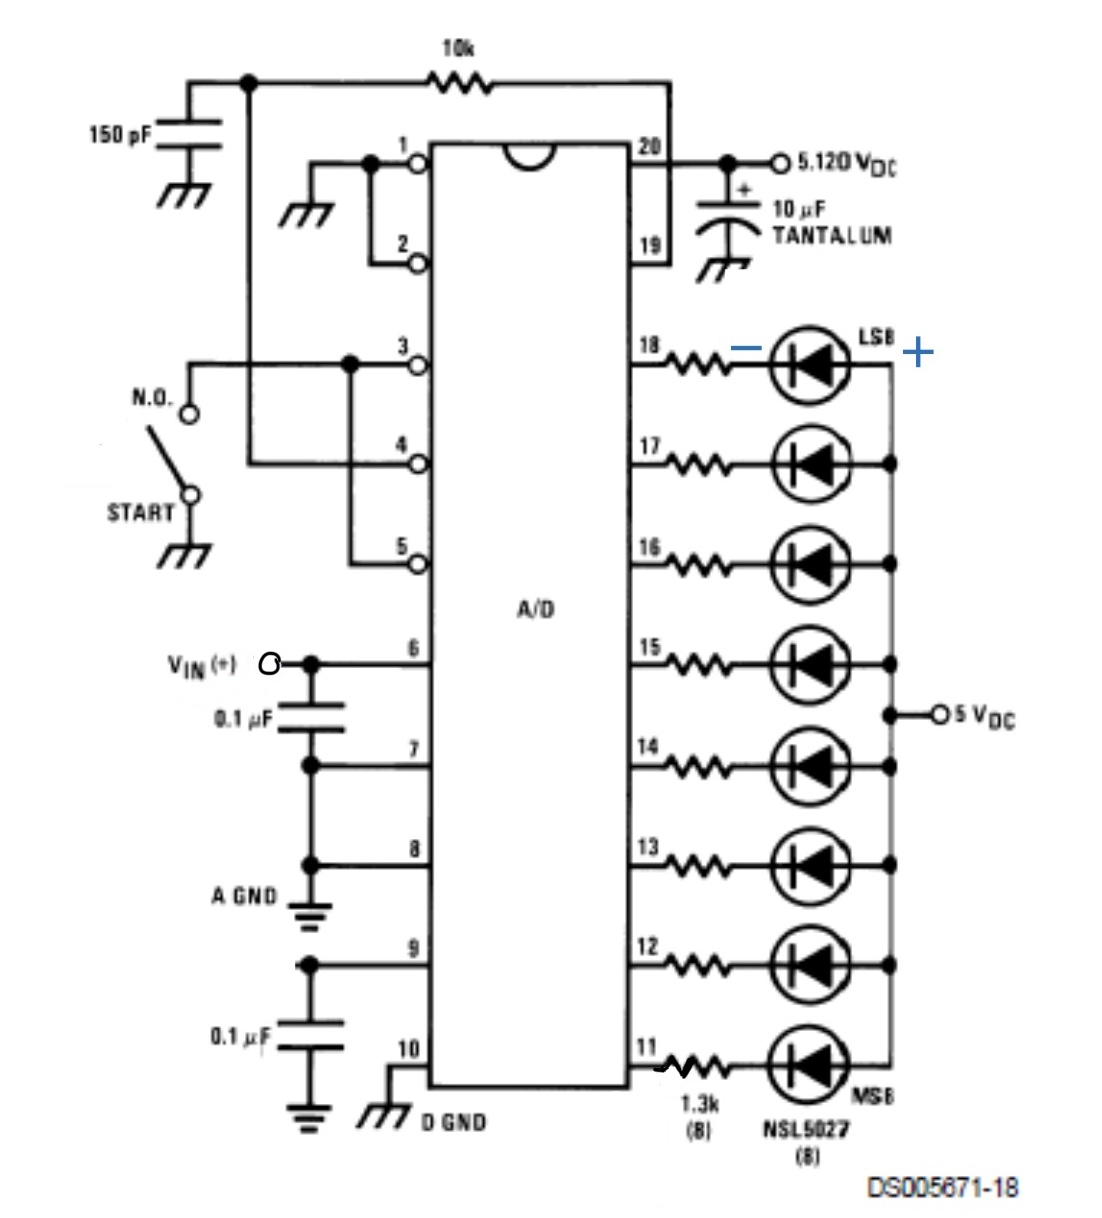
\includegraphics[height=7cm]{images/Schaltungsskizze-versuch-eins.jpg} 
	\caption[]{Schaltungsskizze Versuch 1}
\end{figure}

Zunächst einmal die Schlatungsskizze (Abbildung 2.1) für unseren Versuchsaufbau.

Aufgrund des Fehlen des Schalters haben wir diesen durch ein Kabel ersetzt, welches 
durch einstecken in das Steckbord den Schalter simuliert. \par

Man geht zunächst einmal davon aus, dass die Clockfrequenz des ADC 600 kHz beträgt.\par
Bei der Verschaltung sollte man beachten, dass die Eingangspins 1 - 5, 10, 19 und 20 
haben digitale Referenzwerte, wobei die Eingangspins 6 - 9 haben analoge Referenzwerte.\par
Der V(+)-Eingang muss mit einem Schutzwiderstand 1 k\textOmega  gegen Überspannungen 
und mit einem 0.1 \textmu F gegen Einstreuungen versehen werden. \par

Die Betriebs- und Eingangsspannungen werden mit Hilfe des \acs{DMM} gemessen, um sie möglichst 
genau zu bestimmen.\par
Das Bitmuster wird von den \acs{LED}s in binärer Darstellung abgelesen. Ein \acs{LSB} beträgt 20 mV.\par
Die Versorgungsspannung für den Versuch liege bei 5,120V. Diese definiert den 
Eingangsspannungsbereich U\textsubscript{in}: 0 bis 5,120 V. \newline


Die Schaltung wurde aufgebaut und von einem Betreuer überprüft.
\begin{figure}[H]
	\centering
	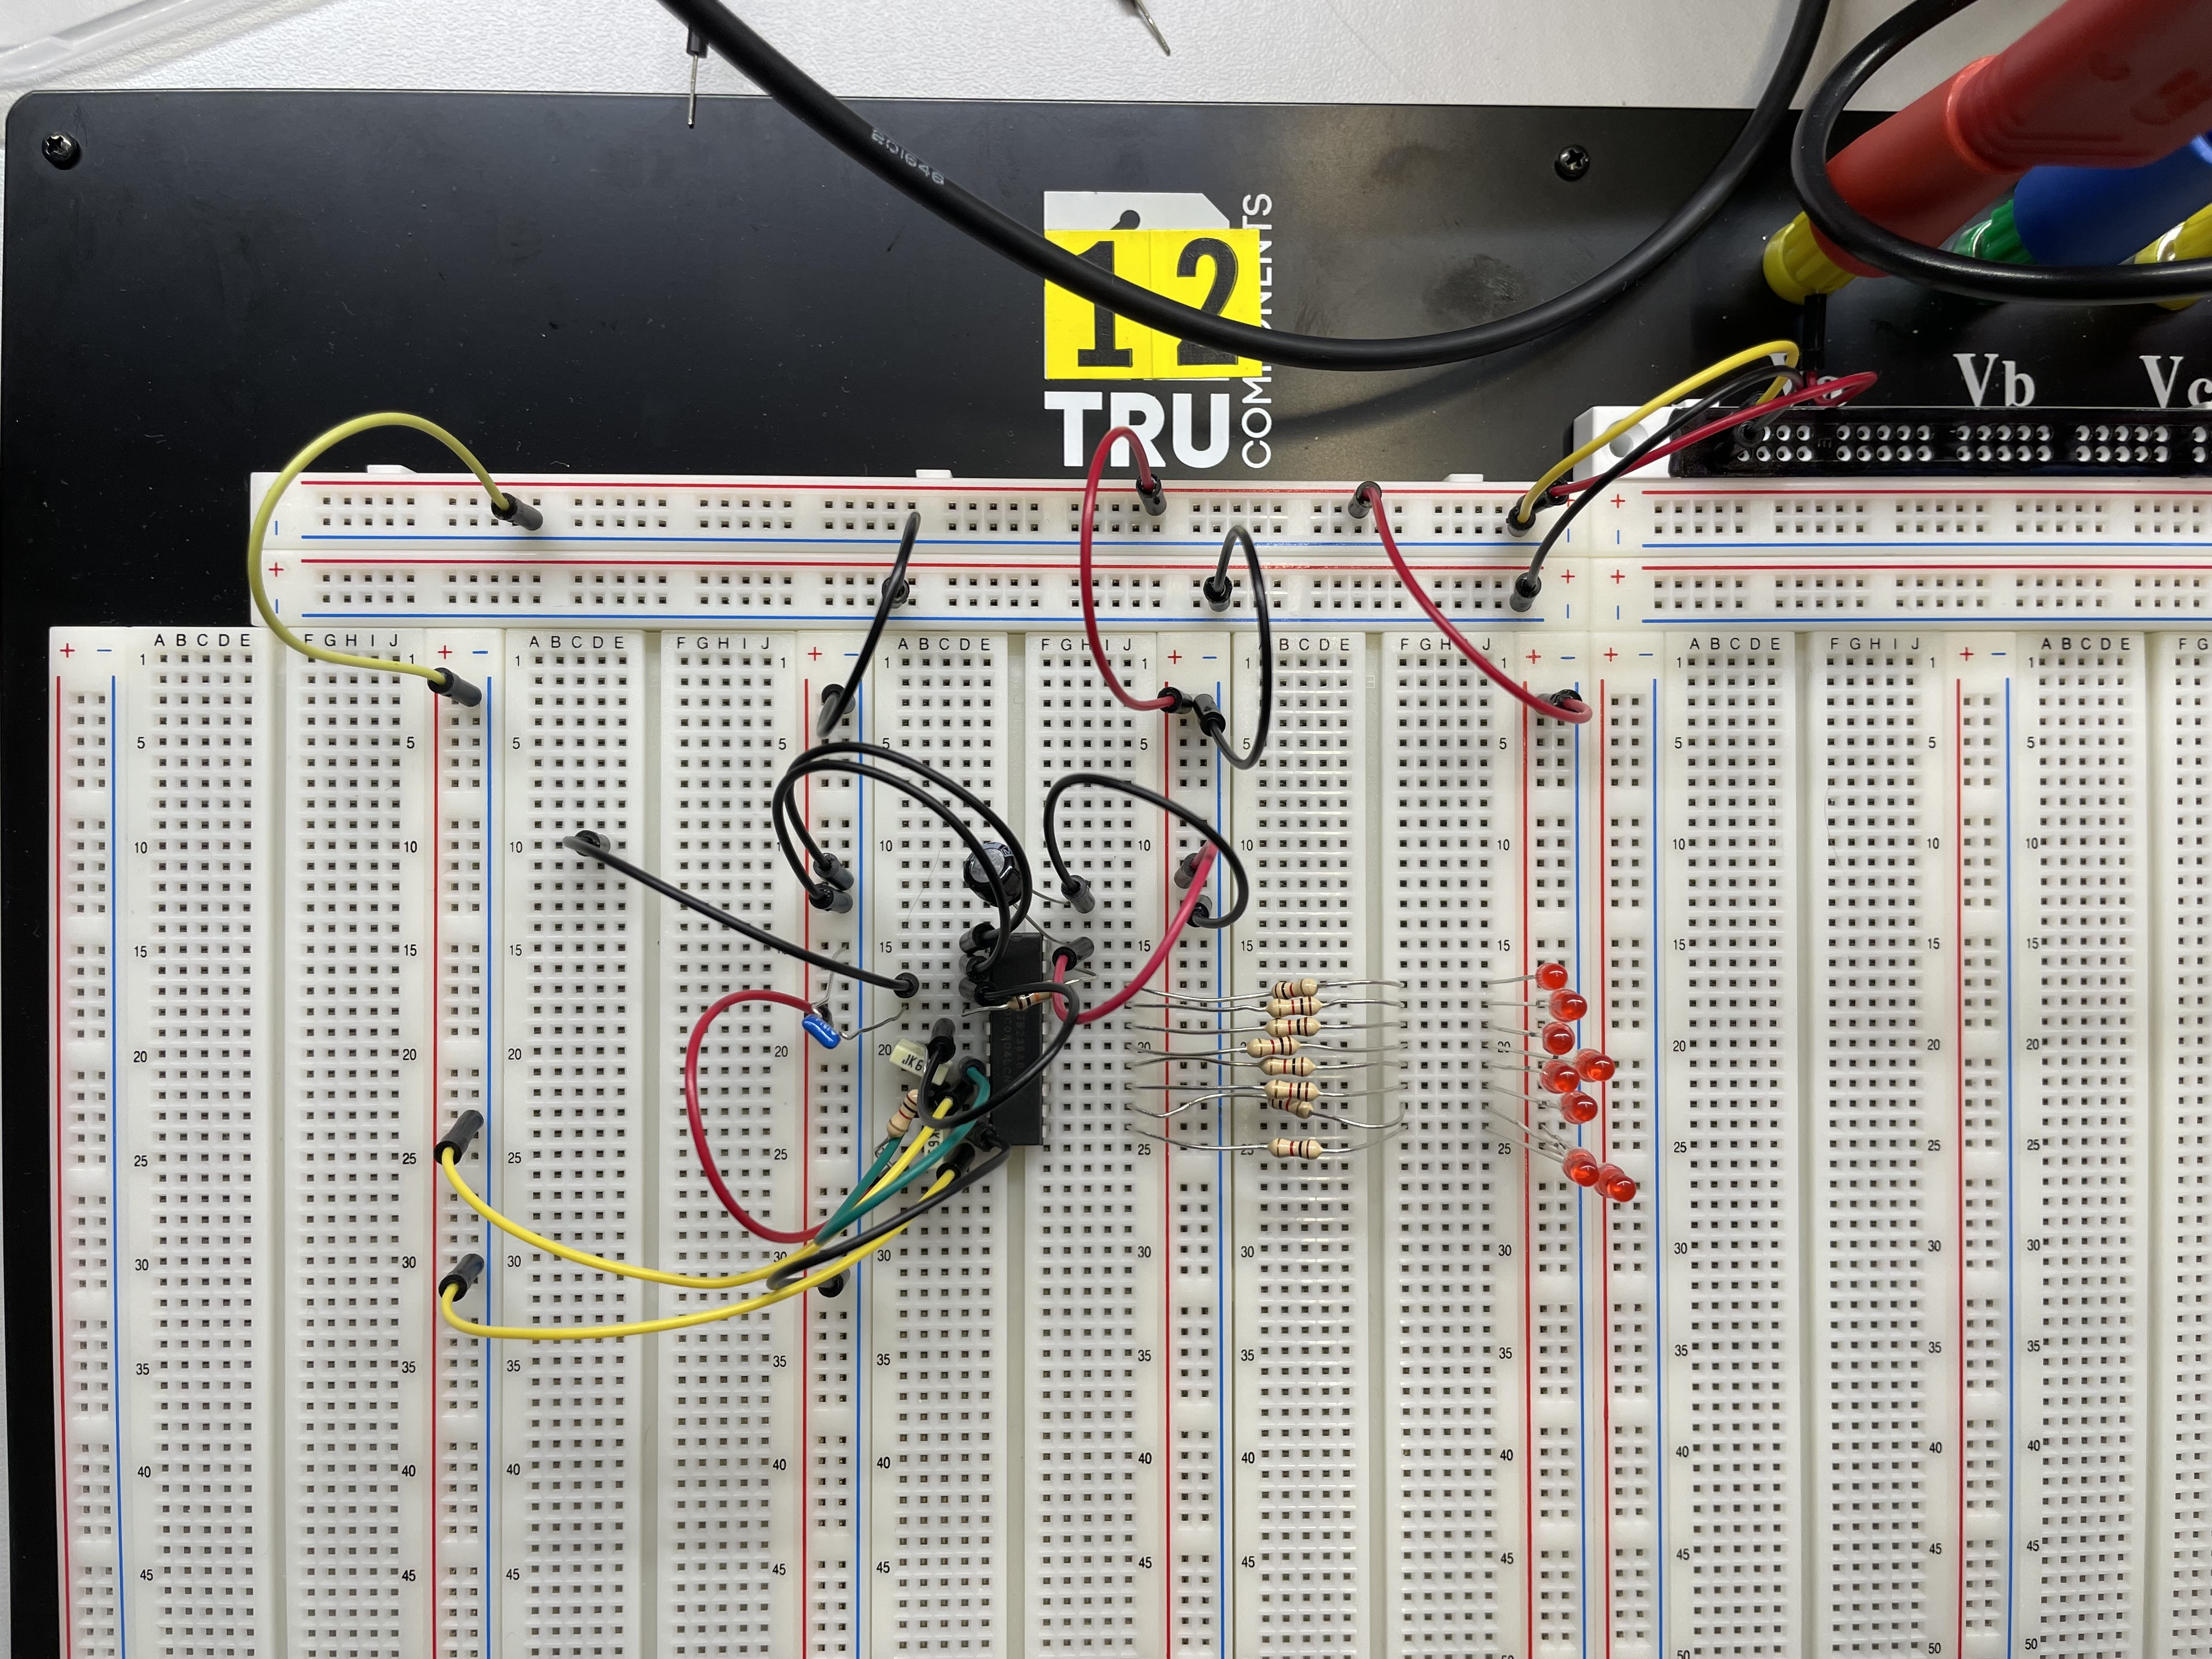
\includegraphics[height=7cm]{images/Schaltungsaufbau-versuch-eins.jpeg} 
	\caption[]{Schaltungsaufbau Versuch 1}
\end{figure}

Der digitale Output der Schaltung wird von den \acs{LED}s in Abbildung 2.2 dargestellt.
Bei der Inbetriebnahme wurde festgestellt, dass die Signale invertiert sind, 
und der Zustand An einer Null entspricht, der Zustand Aus - einer Eins.

\section{Integrale Nichtlinearität}


\begin{table}[H]
	\centering
	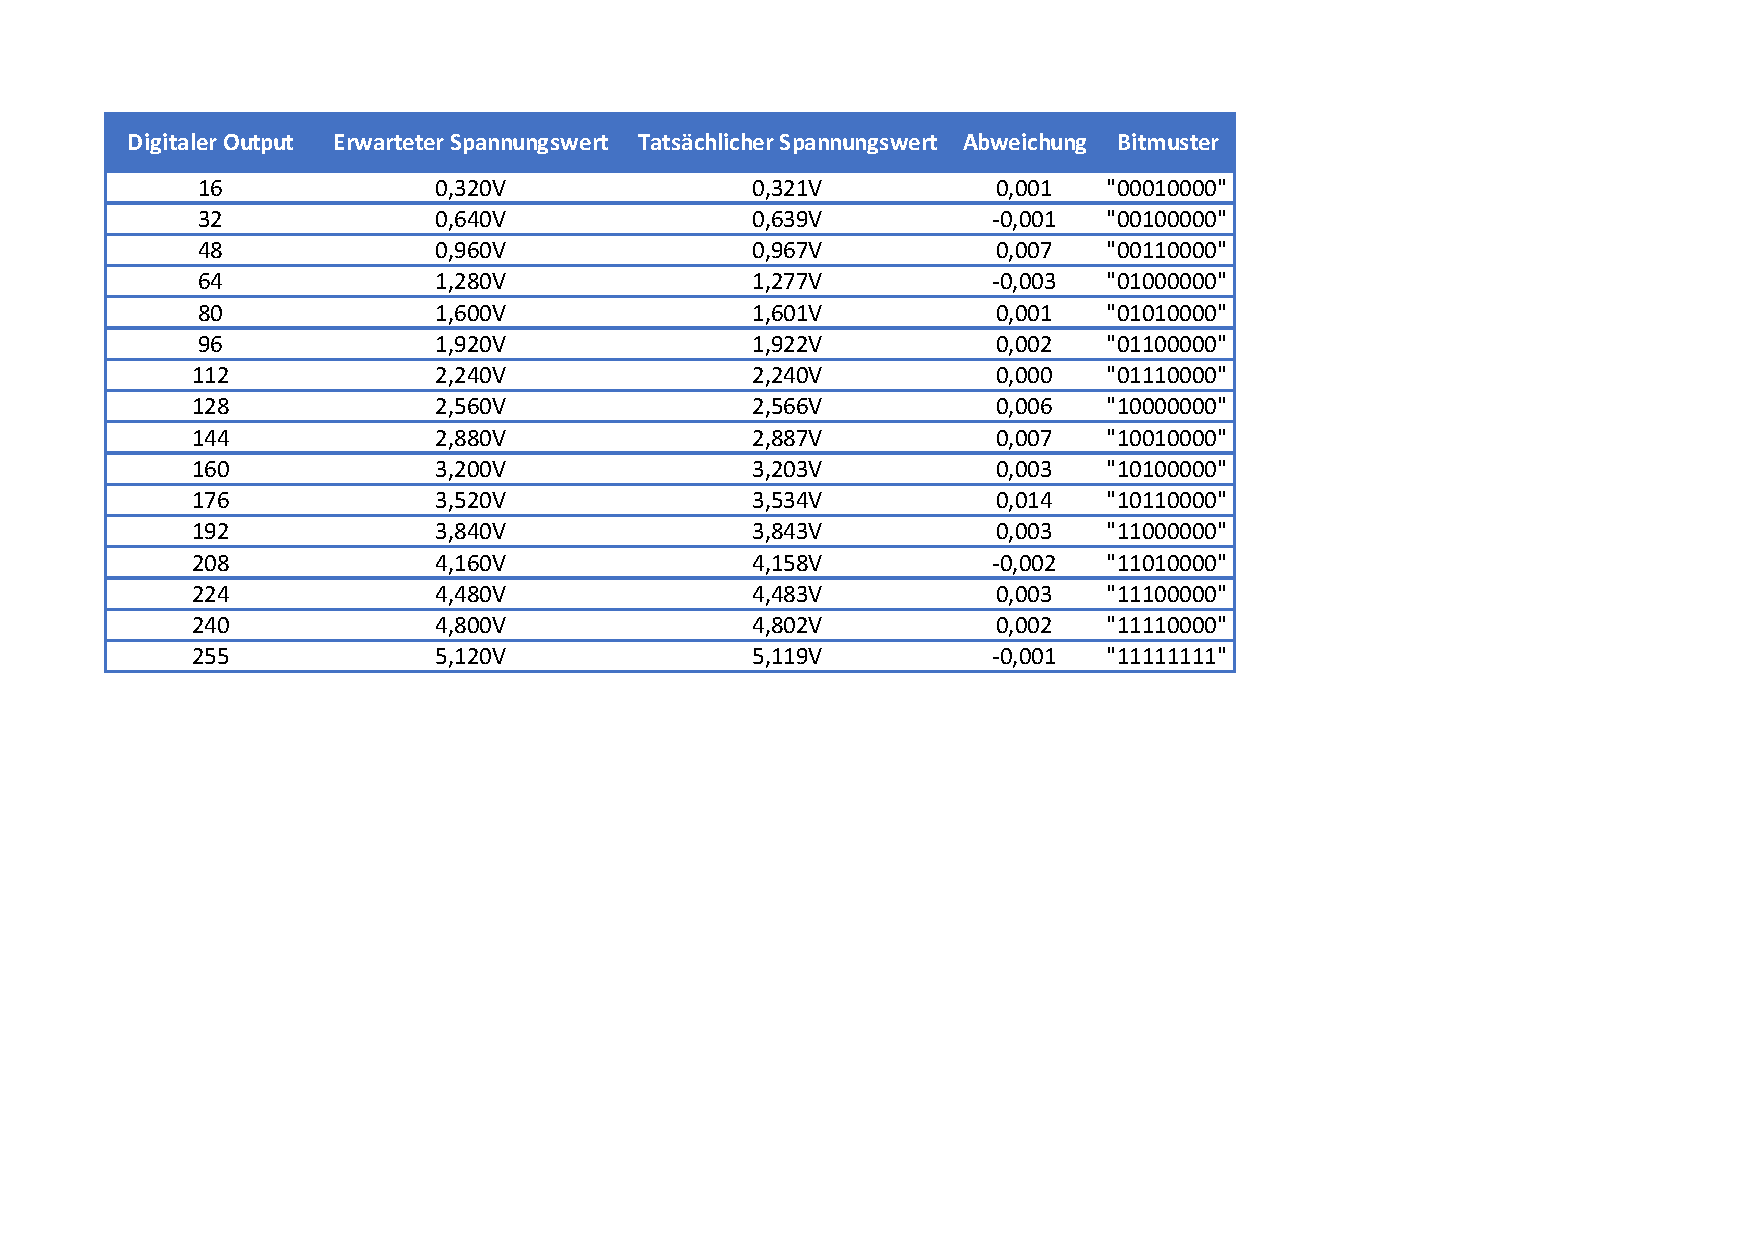
\includegraphics[height=7cm]{images/Versuch-1d.pdf} 
	\caption[]{Ergebnisse Versuch 1d}
\end{table}

TEXT EINFUGEN

\section{Differentiale Nichtlinearität}
\section{Konversionszeit}
